%% LyX 2.1.4 created this file.  For more info, see http://www.lyx.org/.
%% Do not edit unless you really know what you are doing.
\documentclass[english]{article}
\usepackage[T1]{fontenc}
\usepackage[latin9]{inputenc}
\usepackage{float}
\usepackage{graphicx}
\usepackage{babel}
\begin{document}
\begin{abstract}
Simultaneous sensor and actuator placement for identification and
containment of contaminants in a water distribution network.
\end{abstract}

\section{Scenario}


\subsection{Given}

Specification of water distribution network -- vulnerable nodes, demand
nodes, the adjacency matrix.

Time-delay in sensors of contaminant sensing, etc. can be added onto
this work without much hassle, and are ignored.


\subsection{Requirements to be satisfied}

To find distribution of sensors on nodes and actuators on edges such
that the vulnerable node can be identified and the contaminant can
be prevented from reaching the demands.




\section{Previous work}

Sensor placement using the principle that there must exist a unique
non-zero set of sensors for each set of vulnerable nodes that can
be affected.

Actuator placement on edges to achieve a balanced min-cut, between
the sensor nodes and demands.


\section{Hypotheses}

Simultaneous sensor and actuator distribution can be achieved and
is more efficient -- these are dependant problems.


\section{Method}

We first develop an algorithm and formulation for each case, implement
in MATLAB for cases, compare with results from previous work.


\section{Implementation}


\subsection*{Case 1: Shutting the network effectively stops the contaminant beyond
the actuator too.}

In this simpler case, there are no additional constraints on the actuator
placement problem beyond the (balanced) min-cut of the entire graph.

As long as the sensor network can detect the contaminant before it
reaches the demands and the actuation can happen simultaneously, the
requirements are satisfied.


\subsection*{Case 2: The contaminant contained only in the vulnerable side of
actuator network}

This case is not trivial as the positions of the sensors must be used
as input, i.e ensuring they are on the vulnerable side.

Formalism as binary integer optimization problem:

\begin{eqnarray*}
min & (\sum x_{i}+\sum y_{i}+\sum z_{i})\\
sub\\
\mathbf{A}\left[\begin{array}{c}
\mathbf{x}\\
\mathbf{y}\\
\mathbf{z}
\end{array}\right] & \geq & \mathbf{b}\\
\mathbf{A_{eq}}\left[\begin{array}{c}
\mathbf{x}\\
\mathbf{y}\\
\mathbf{z}
\end{array}\right] & = & \mathbf{b_{eq}}
\end{eqnarray*}


Where $x_{i}$ is 1 if there exists a sensor at $i^{th}$node, 0 otherwise.

$y_{i}$ is 1 if $i^{th}$node is in the demands side of the actuators,
0 otherwise. 

$z_{i}$ is 1 if there exists an actuator at $i^{th}$edge, 0 otherwise.

After adding constraints from each of the sub-problems, the only thing
left to do to enforce containment is to add constraints reflecting
it. Our aim is to force whatever partitioning to happen in the region
farther away from the contaminant than the sensor nodes. So we use
shortest path lengths from all the vulnerable nodes (simulating an
attack on all of them) to all the nodes in the graph to model ``farther
away''. There are still problems associated with this approach, which
I'm working on now.

For example, take the graph generated by \emph{adjGraph = sparse({[}1
1 2 2 2 3 3 4 5{]},{[}2 3 4 5 3 4 5 6 6{]},{[}2 2 1 1 1 1 1 2 2{]},6,6);}

\begin{figure}[H]
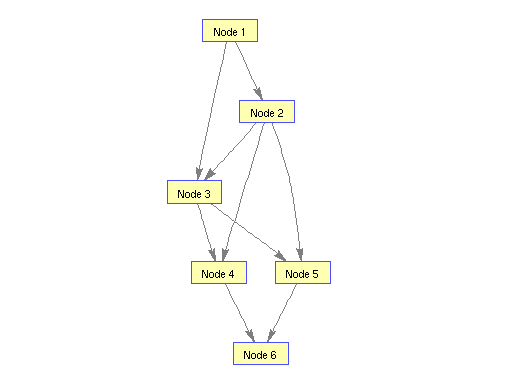
\includegraphics{testGraph}\caption{The test graph}
\end{figure}


I'm currently working on implementing this in MATLAB.
\begin{thebibliography}{1}
\bibitem{key-1} V. Reddy, 2015 - Sensor network design for contaminant
detection and identification in water distribution networks.

\bibitem{key-2}\end{thebibliography}

\end{document}
